\chapter{Redes Neuronais Artificiais}
\label{chp:rna}

\section{Descrição geral}
\label{sec:RNA-Descricao}

Apresentando-se como uma abordagem de \textit{machine learning}, os algoritmos de redes neuronais artificias (RNAs) baseiam-se num sistema conexionista, inspirado no funcionamento da estrutura cerebral humana.

Estas técnicas recorrem a uma topologia em rede para receber informações que, após processadas, influenciam o estado interno de cada neurónio da rede.
O conhecimento é assim adquirido através do ambiente por um processo iterativo de aprendizagem. 
Este conhecimento é armazenado nas conexões da rede, através de uma adaptação dos pesos dos neurónios -ou nodos- ao longo de um processo de aprendizagem. 

Independente do contexto, uma rede neuronal apresenta uma arquitetura genérica (Figura \ref{fig:arquiteturas}), normalmente composta pelas seguintes camadas \cite{CortezNevesANN, ann-agility}: 
\begin{itemize}
    \item \textbf{Camada de entrada}, na qual é recebida a informação a analisar. 
    Apesar dos dados serem normalmente obtidos através de um dataset pré preparado, esta camada pode ser vista como a comunicação da rede com o ambiente, como forma de percecionar e obter dados. 
    
    É assim uma camada sem antecessor, servindo como uma interface para alimenta a rede com nova informação. 
    
    \item \textbf{Camadas intermédias}, que desempenham a tarefa de processamento dos dados de entrada, com base num determinado paradigma de aprendizagem. 
    
    \item \textbf{Camada de saída}, onde se devolvem os resultados do processo de aprendizagem da rede. 
    
    O número de nodos de saída está diretamente relacionado com o número de parâmetros que são previsto pela rede num determinado contexto. 
\end{itemize}

Alguns dos benefícios das redes neuronais, comparativamente a outros processos de \textit{Machine Learning}, estão associados ao seu puder de processamento. Esta capacidade deve-se essencialmente à sua estrutura, que permite executar um ambiente extremamente paralelo.
Além deste fator, apresentam ainda outras características de relevo, nomeadamente \cite{ann-agility}  \cite{CortezNevesANN} \cite{Haykin-ANN}:
\begin{itemize} 
    \item \textbf{Generalização}: No final do processo de aprendizagem, a rede é capaz de descrever um universo completo, através de uma aprendizagem prévia com algumas das suas partes. 
    Além disto, devido à sua robustez, as RNAs são ainda capazes de processar ruído ou informação incompleta, conseguindo generalizar a informação que analisam na fase de treino para novos casos futuros. 
    
    \item \textbf{Não linearidade}: Além de problemas simples, estes algoritmos apresentam-se capazes de analisar características não lineares, através da interconexão de diferentes neurónios e uso de diferentes funções de ativação; 
    
    \item \textbf{Relação entre input-output}: Quando aplicadas num contexto de aprendizagem supervisionada, com um conjunto de input de treino e um dataset de output esperado, as redes neuronais são capazes de gerar resultados satisfatórios de classificação;
    
    \item \textbf{Adaptação}: Uma das principais características das RNAs reside na sua capacidade de adaptação, útil em ambientes com dados desconhecidos ou em falta. 
    
    Os pesos atribuídos a cada neurónio são capazes de ser adaptar, conforme o domínio sobre a qual a rede se encontra a ser treinada. Alem disto, a sua topologia pode também alterar-se de acordo com as mudanças do ambiente, criando ou reduzindo o número de ligações entre nodos. 

    Desta forma, no final do processo de aprendizagem, uma RNA é capaz de generalizar novos casos à sua capacidade de raciocínio. 
    
    \item \textbf{Tolerância a falhas}: Devido à sua topologia, as RNAs permitem um elevada tolerância a falhas. 
    A falha de um neurónio pode ser atenuada pela marcação do peso dos seus axónios como zero, simulando assim o desaparecimento das ligações para aquele neurónio. 
    
    A falha de um neurónio leva ao reajustamento dos restantes, levando a uma degradação gradual e suave da rede, em caso de desativação de algumas conexões entre neurónios. 
\end{itemize}


\section{Neurónio Artificial}
\label{sec:Neuronio}

Cada camada de uma RNA é composta por um conjunto de neurónios, identificados pelos nodos da topologia da rede. 
Um neurónio pode ser visto como uma unidade de processamento da rede, recebendo ligações de outro neurónios e unindo-se a outros nodos da rede semelhantes a si. 

As ligações entre neurónios são designadas por axónios, tal como na estrutura biológica do cérebro e, têm a si associadas um peso. Este peso pode, numa interpretação simples, ser visto como a importância da informação que aquele axónio envia a um neurónio.
O peso de cada axónio é regulado ao longo do processo de aprendizagem, levando a uma generalização da topologia da rede aos dados, até se obter um resultado coerente com os esperados no contexto. 
A transmissão de informação entre os nodos é conseguida através de sinapses, novamente seguindo a nomenclatura biológica. 

Ao longo do processo de evolução da rede, os neurónios vão atualizando o seu estado, sendo este normalmente representado por um valor numérico entre \textit{[0, 1]}.
De uma forma geral, o estado interno de um neurónio é caracterizado por:
\begin{itemize} 
    \item Um \textbf{conjunto de ligações}, cada uma com o seu próprio peso. 
    Ao longo da evolução da rede, o sinal propagado por um determinado axónio é multiplicado pelo peso do mesmo, resultando assim na excitação -ou inibição- do nodo;

    \item Um \textbf{Integrador}: Apresenta-se como uma função de redução, que simplifica a influencia das N conexões de entrada de um neurónio para um único valor. 
    
    Geralmente, o integrador realiza apenas o somatório $(\sum)$ dos valores recebidos pelas N ligações de entrada, multiplicados pelo peso da respetiva ligação;
    
    \item A \textbf{Função de Ativação}: Determina o valor de saída do neurónio, de forma a restringir o valor de saída do neurónio para um determinado valor finito. 
    Este valor é normalmente calculado através do mapeamento do valor do integrador para uma determinada função não linear. De referir que a escolha da função de ativação tem uma influência direta e bastante significativa na capacidade de aprendizagem da rede.  
    
    Algumas das principais funções são a função binária (degrau), linear ou funções do tipo \textit{sigmoide}. \cite{ANN-chemiProb}
    Em pesquisas recentes, foi ainda apresentada a função designada por \textit{ReLU}. (Figura \ref{fig:act-func}) Esta função, explorada pelos investigadores da \textit{Google Brain Team}, apresenta algumas vantagens face a implementações com a função \textit{sigmoide}.

\end{itemize}

\begin{figure}
    \hspace{-0.2in}
    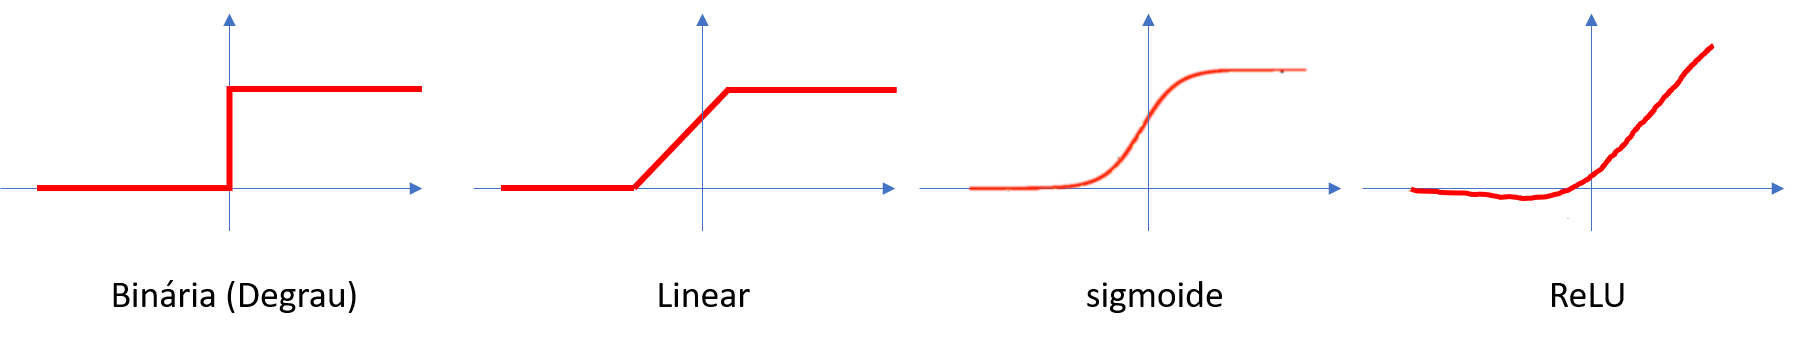
\includegraphics[scale=0.53]{Imagens/actfun.png}
    \caption{Exemplos de diferentes tipos de funções utilizadas como função de ativação dos neurónios.}
    \label{fig:act-func}
\end{figure}

\section{Arquiteturas da Rede }
\label{sec:Arquiteturas}

A arquitetura de uma rede neuronal artificial especifica a quantidade de neurónios (nodos) que a mesma possui e, de que formas estes se relacionam e interligam entre si.
A arquitetura pode ser visualizada na forma de grafos, no qual as ligações entre os nodos são orientadas. 

De uma forma geral existem três tipos distintos de topologia, sendo que quanto mais complexa a arquitetura de uma RNA, maior a sua capacidade para lidar com problemas mais complexos. 

\begin{itemize}
    \item \textbf{\textit{Single Layer Feedforward}}: As ligações da rede seguem apenas uma direção. Nesta arquitetura não existem camadas intermédias, existindo apenas as camadas de \textit{input} e \textit{output}. 
    
    A partir de um nodo de entrada existem apenas ligações divergentes (1 para N)  e os nodos de saída apresentam ligações convergentes (N para 1). Esta topologia representa as arquiteturas inicias das RNAs. (Figura \ref{fig:arquiteturas}-a)
    
    \item \textbf{\textit{Multi-Layer Feedforward}}: Seguindo os mesmos conceitos da arquitetura anterior, as RNAs \textit{multi-layer} permitem a definição de uma ou mais camadas intermédias. 
    Embora esta relação não seja linear, a adição de camadas intermédias a uma rede permite aumentar a sua capacidade de aprendizagem, podendo assim lidar com funções e relações entre os dados mais complexas. 
    
    Estas redes são assim úteis em contextos onde existe um grande número de dados de input, sobre os quais se espera observar alguma relação ou padrões gerais. Contudo, o aumento do número de camadas de uma rede neuronal, leva a um aumento exponencial do seu tempo de aprendizagem. (Figura \ref{fig:arquiteturas}-b)
    
    Neste tipo de arquiteturas, o algoritmo de \textit{Back-Propagation} é um dos principais métodos de aprendizagem. Este método calcula a contribuição do erro para cada um dos nodos da rede, ajustando o peso de cada nodo com base no erro calculado (Secção \ref{sec:backProp}). 

    \item \textbf{Redes recorrentes}: Numa sucessão à arquitetura anterior, as RNAs baseadas em  redes recorrentes permitam a existência de conexões de um nodo para si próprio. A ligação de um neurónio para si próprio permite a introdução de conceitos de “memória” no próprio nodo. 
    
    Além deste fator, um neurónio pode ainda ligar-se a outros nodos de camadas anteriores ou da própria camada, permitindo assim a existência de ciclos na estrutura. (Figura \ref{fig:arquiteturas}-c)
\end{itemize}

\begin{figure}
    \hspace{-0.2in}
    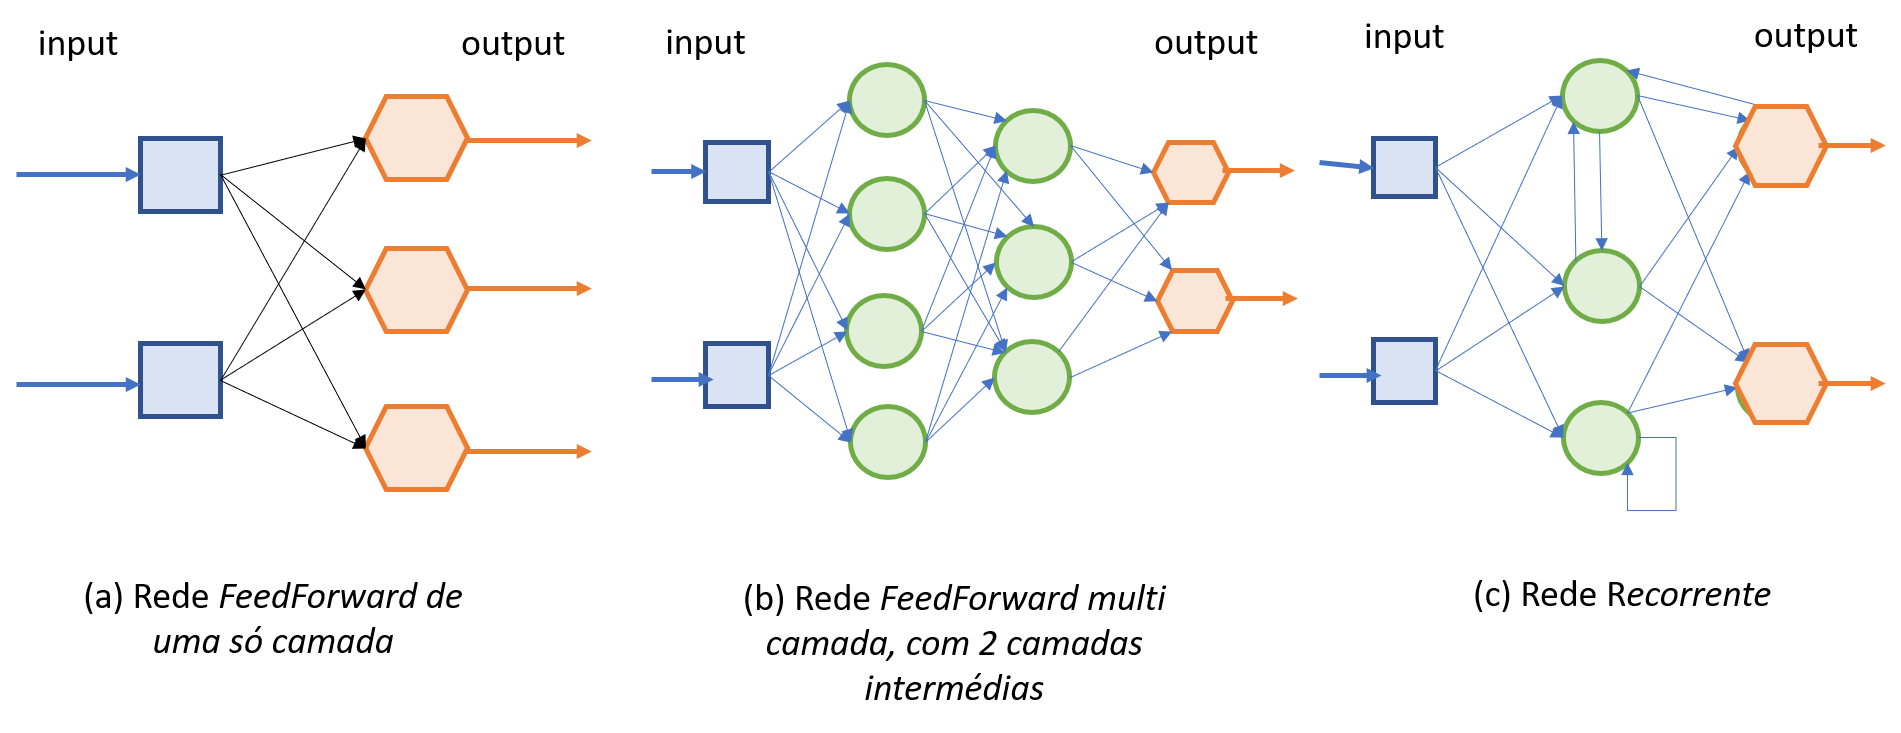
\includegraphics[scale=0.5]{Imagens/topos.png}
    \caption{Exemplos de algumas topologias de arquiteturas de RNAs}
    \label{fig:arquiteturas}
\end{figure}

\section{\textit{Back-Propagation}}
\label{sec:backProp}

Associado ao método de aprendizagem do Gradiente Descendente, o algoritmo de \textit{Back-Propagation} é um dos algoritmos mais utilizados no paradigma de aprendizagem supervisionada de redes neuronais artificiais. 

Regras de aprendizagem do tipo Gradiente Descendente baseiam-se na diminuição de um erro, sendo este estimado entre um valor pretendido e um valor obtido pela previsão da rede. \cite{Haykin-ANN}
Para cada estado do processo de evolução da rede, o objetivo prende-se com a minimização de uma função de custo, definida em termos do valor de erro. 

Este processo de avaliação é descrito pela Equação \ref{eq1}, onde $\eta$ é a taxa de aprendizagem e $\Delta \epsilon$ a diferenças entre o valor esperado e o valor obtido para uma dada entrada (gradiente da função de custo).  

\begin{equation}
    \label{eq1}
    \Delta w = \eta \Delta \epsilon
\end{equation}

No caso especifico do algoritmo de \textit{Back-Propagation}, a sua implementação segue os seguintes passos:
\begin{itemize}
    \item Antes de se iniciar o treino, são atribuídos valores aleatórios aos axónios da arquitetura, marcando assim o peso inicial de cada ligação; 
    
    \item Iniciado o treino, os valores (vetores entrada) fornecidos aos nodos de input  vão-se propagando para a frente, até chegarem aos nodos de saída. Chegando à camada final, é calculado o erro entre o valor obtido pela rede e o valor esperado; 
    
    \item O referido erro é propagado para as camadas anteriores, desde os nodos de saída até aos aos nodos da camada de \textit{input}. Esta retro propagação leva ao ajustamento dos pesos de cada nodo segundo a regra de \textit{Widrow-Hoff} Equação \ref{eq1};
    
    \item Este processo é repetido para cada iteração. A fase de treino termina quando forem cumpridos os critérios de paragem definidos.
\end{itemize}
